\documentclass[a4paper,10pt]{article}
\usepackage{longtable}
\usepackage[utf8]{inputenc}
\usepackage{url}
\usepackage{listings}
\usepackage{color}
\usepackage{verbatim}
\definecolor{grey}{rgb}{0.9,0.9,0.9}
\usepackage{float}
\usepackage{graphicx}
\usepackage{fancyhdr}
\pagestyle{fancy} % voir si laisse ce style ou pas ?
\usepackage{rotating}
%\usepackage[top=2.5cm,bottom=2.5cm,right=2.5cm,left=2.5cm]{geometry}
\usepackage[right=4cm,left=4cm]{geometry}
\lstset{
language=Python,
basicstyle=\footnotesize\fontfamily{pcr},
backgroundcolor=\color{grey},
numbers=left,
numberstyle=\tiny,
numbersep=5pt,
showstringspaces=false,
tabsize=2,
breaklines=true,
morekeywords={elsif}
}
\usepackage{hyperref}
\hypersetup{
	bookmarks=true,         % show bookmarks bar? 
	unicode=true,         	% non-Latin characters in Acrobat’s bookmarks
	pdftoolbar=true,        % show Acrobat’s toolbar?
	pdfmenubar=true,        % show Acrobat’s menu?
	pdffitwindow=false,     % window fit to page when opened
	pdfstartview={FitH},    % fits the width of the page to the window
	pdftitle={INFO-F403 : rapport},
    pdfauthor={Chapeaux Thomas, Dagnely Pierre},
    colorlinks=true,       % false: boxed links; true: colored links
    linkcolor=black,          % color of internal links
    citecolor=green,        % color of links to bibliography
    filecolor=magenta,      % color of file links
    urlcolor=cyan           % color of external links
}
\let\oldtabular=\tabular
\def\tabular{\footnotesize\oldtabular}



% Title Page
\title{INFO-F403 Introduction to Language Theory and Compilation}
\author{Chapeaux Thomas\\Dagnely Pierre}

\begin{document}
\maketitle


\pagebreak


\renewcommand{\contentsname}{Table des matières}
\tableofcontents
%\pagebreak

\section{Introduction}

Le but du projet était de construire un compilateur d'une version simplifiée de Perl en ASM/ARM devant tourner dans une architecture Android. Nous avons choisi d'implémenter notre compilateur en Python 2.7\footnote{\url{http://www.python.org/}}.\\

La première partie de ce rapport se concentrera sur l'analyse du langage, c'est-à-dire la définition des tokens et de la grammaire LL(1) correspondante, ainsi que la table d'action et les contraintes que nous avons imposé lors de la transformation en LL(1). Ensuite, nous décrirons les outils que nous avons implémentés (scanner et parser) qui transforment un fichier .perl en un AST et finalement, nous expliquerons la génération du code ASM/ARM depuis celui-ci.

%%%%%%%%%%%%%%%%%%%%%%%%%%%%%%%%%%%%%%%%%%%%%%%%%%%%%%%%%%%%%%%%%%%%%%%%%%%%%%%%%%%%%%%%%%%%%%%%%%%%%%%%%%%%%%%%%%%%%%%%%%%%%%%%%%%%%%%%%%%%%%%%%%%%
%%
%%
%%
%%					CHAP 1 : grammaire
%%
%%
%%
%%%%%%%%%%%%%%%%%%%%%%%%%%%%%%%%%%%%%%%%%%%%%%%%%%%%%%%%%%%%%%%%%%%%%%%%%%%%%%%%%%%%%%%%%%%%%%%%%%%%%%%%%%%%%%%%%%%%%%%%%%%%%%%%%%%%%%%%%%%%%%%%%%%%%%%


\section{La grammaire}

\subsection{Définition des unités lexicales}

La première étape de ce projet consiste à récupérer et analyser toutes les unités lexicales du langage, c'est à dire tous les "composants" possibles.\\
Pour cette partie nous nous sommes basés sur la grammaire complète donnée au début du projet.\\
Le scanner utilise aussi cette grammaire, mais les étapes suivantes ne se basent plus que sur la grammaire simplifiée, ainsi certaines unités lexicales ne sont pas supportés par notre compilateur : seul ceux cités dans la grammaire le sont.\\
\begin{tabular}{cc}

\begin{tabular}{|c|l|}
\hline
unité lexicale		& expression régulière \\ \hline
INT					& ([0-9])* \\ \hline
FLOAT				& ([0-9])*.DOT.([0-9])* \\ \hline
BOOL				& (0+1+true+false+'') \\ \hline
STRING				& '.([A-Za-z]+[0-9])*.'  \\ \hline
FAC					& ! \\ \hline
MUL					& * \\ \hline
DIV					& / \\ \hline
MINUS				& - \\ \hline
ADD					& + \\ \hline
LT					& $<$ \\ \hline
GT					& $>$ \\ \hline
LE					& $<=$ \\ \hline
GE					& $>=$ \\ \hline
EQUIV				& == \\ \hline
DIF					& != \\ \hline
AND					& \&\& \\ \hline
OR					& $||$ \\ \hline
NOT					& not \\ \hline
LT-S				& lt \\ \hline
GT-S				& gt \\ \hline
LE-S				& le \\ \hline
GE-S				& ge \\ \hline
EQ-S				& eq \\ \hline 
NE-S				& ne \\ \hline
\end{tabular}

&

\begin{tabular}{|c|l|}
\hline
unité lexicale		& expression régulière \\ \hline
EQUAL				& = \\ \hline
DOT					& . \\ \hline
SEMICOLON			& ; \\ \hline
COMA				& , \\ \hline
OPEN-PAR			& ( \\ \hline
CLOSE-PAR			& ) \\ \hline
OPEN-BRAC			& \{ \\ \hline
CLOSE-BRAC			& \} \\ \hline
OPEN-COND			& IF \\ \hline
CLOSE-COND 			& ELSE \\ \hline
ADD-COND			& ELSIF \\ \hline
NEG-COND			& UNLESS \\ \hline
RET					& return \\ \hline
FUNCT-DEF			& SUB \\ \hline
ID					& STRING \\ \hline 
FUNCT-NAME			& \&.STRING \\ \hline
PERL-DEF			& defined  \\ \hline
PERL-INT			& int  \\ \hline
PERL-LENG			& length  \\ \hline
PERL-SCAL			& scalar  \\ \hline
PERL-SUBS			& substr  \\ \hline
PERL-PRIN			& print\\ \hline
COMM				& \#.STRING \\ \hline
VARIABLE			& \$.STRING \\ \hline


\end{tabular}
\end{tabular}


\subsection{Modification}\label{sct:gramModif}

	
Nous nous sommes basés sur la grammaire simplifiée afin de faciliter certaines étapes du projet, la grammaire complète présentant certaines difficulté. Nous avons ajoutés la grammaire simplifiée initiale en annexe \ref{gramm-init}, ainsi ne sont reprise ci-dessous que les règles après modifications.\\
Mais un numéro de ligne indique à chaque fois quelle règle a été modifiée.\\
~\\
Pour rendre cette grammaire LL(1), nous avons suivi plusieurs étapes : 
\subsubsection{Suppression des symboles inutiles}

	On doit commencer par retirer tous les symboles non-productifs et tous les symboles inaccessibles.\\
	Ici tous les symboles sont utiles, on ne modifie donc pas la grammaire

\subsubsection{Gestion des priorités et associativité}
	On veut retirer les ambiguïtés liées aux priorités et à l'associativité.\\
	Cela ne concerne que la règle EXP (29-36), on la transforme donc en respectant les règles de priorités et d'associativités habituelles : \\

	\begin{center}\begin{tabular}{rl}
		$<$EXP$>$			& $\rightarrow$ $<$EXP$>$ equiv $<$EXP-2$>$ \\
							& $\rightarrow$ $<$EXP$>$ gt $<$EXP-2$>$ \\ 
							& $\rightarrow$ $<$EXP-2$>$ \\
					
		$<$EXP-2$>$			& $\rightarrow$ $<$EXP-2$>$ add $<$EXP-3$>$   \\
							& $\rightarrow$ $<$EXP-2$>$ minus $<$EXP-3$>$ \\ 
							& $\rightarrow$ $<$EXP-3$>$ \\

		$<$EXP-3$>$			& $\rightarrow$ $<$EXP-3$>$ mul $<$SIMPLE-EXP$>$  \\
							& $\rightarrow$ $<$EXP-3$>$ div $<$SIMPLE-EXP$>$\\ 
							& $\rightarrow$ $<$SIMPLE-EXP$>$ \\					
	\end{tabular}\end{center}

\subsubsection{left factoring}
	On modifie toute règle ayant un même premier symbole généré.\\
	Cela ne concerne que les règles EXP, EXP-2, EXP-3 et PROGRAM(1-3) : \\
	Cependant cette étape impacte l'associativité gauche des opérations, afin de résoudre ce problème de la manière la plus simple, nous avons décidé d'imposer l'utilisation des parenthèses dans les calculs.
	\begin{center}\begin{tabular}{rl}
		$<$PROGRAM$>$		& $\rightarrow$ $<$FUNCT-LIST$>$ $<$PROG-TAIL$>$\\
							& $\rightarrow$ $<$INSTRUCT-LIST$>$\\
		$<$PROG-TAIL$>$		& $\rightarrow$ $<$INSTRUCT-LIST$>$\\
							& $\rightarrow$ epsilon\\
							&\\
							&\\
		$<$EXP$>$			& $\rightarrow$ $<$EXP-2$>$ $<$EXP-TAIL$>$ \\

		$<$EXP-TAIL$>$		& $\rightarrow$ equiv $<$EXP-2$>$ $<$EXP-TAIL$>$\\
							& $\rightarrow$ gt $<$EXP-2$>$ $<$EXP-TAIL$>$\\ 
							& $\rightarrow$ epsilon \\
					
		$<$EXP-2$>$			& $\rightarrow$ $<$EXP-3$>$ $<$EXP-2-TAIL$>$ \\

		$<$EXP-2-TAIL$>$	& $\rightarrow$ add $<$EXP-3$>$ $<$EXP-2-TAIL$>$\\
							& $\rightarrow$ minus $<$EXP-3$>$ $<$EXP-2-TAIL$>$\\ 
							& $\rightarrow$ epsilon \\
					
		$<$EXP-3$>$			& $\rightarrow$ $<$SIMPLE-EXP$>$ $<$EXP-3-TAIL$>$ \\

		$<$EXP-3-TAIL$>$	& $\rightarrow$ mul $<$SIMPLE-EXP$>$ $<$EXP-3-TAIL$>$\\
							& $\rightarrow$ div $<$SIMPLE-EXP$>$ $<$EXP-3-TAIL$>$\\ 
							& $\rightarrow$ epsilon \\				
	\end{tabular}\end{center}

\subsubsection{Left recursion}
	Les grammaires LL(k) ne peuvent contenir de règles du type $A \rightarrow A \beta$.\\
	Cela concerne FUNCT-LIST (4-5), ARG-LIST(8-10), INSTRUCT-LIST(11-12) et FUNCT-CALL-ARG(14-16) : \\

	\begin{center}\begin{tabular}{rl}				
					
		$<$FUNCT-LIST$>$		& $\rightarrow$ $<$FUNCT-LIST-BEG$>$ $<$FUNCT-LIST-END$>$\\
		$<$FUNCT-LIST-BEG$>$	& $\rightarrow$ $<$FUNCT$>$ \\
		$<$FUNCT-LIST-END$>$	& $\rightarrow$ $<$FUNCT$>$ $<$FUNCT-LIST-END$>$\\
								& $\rightarrow$ EPSILON \\
								&\\
								&\\

		$<$ARG-LIST$>$			& $\rightarrow$ $<$ARG-LIST-BEG$>$ $<$ARG-LIST-END$>$\\ 
		$<$ARG-LIST-BEG$>$		& $\rightarrow$ variable\\ 
								& $\rightarrow$ epsilon \\
		$<$ARG-LIST-END$>$		& $\rightarrow$ coma variable $<$ARG-LIST-END$>$\\ 
								& $\rightarrow$ epsilon \\
								&\\
								&\\
		$<$INSTRUCT-LIST$>$		& $\rightarrow$ $<$INSTRUCT$>$ semicolon $<$INSTRUCT-LIST$>$\\
								& $\rightarrow$ epsilon\\
								&\\
								&\\

		$<$FUNCT-CALL-ARG$>$	& $\rightarrow$ $<$FUNCT-CALL-ARG-BEG$>$ $<$FUNCT-CALL-ARG-END$>$\\ 
		$<$FUNCT-CALL-ARG-BEG$>$& $\rightarrow$ $<$EXP$>$\\ 
								& $\rightarrow$ epsilon \\
		$<$FUNCT-CALL-ARG-END$>$& $\rightarrow$ coma $<$EXP$>$ $<$FUNCT-CALL-ARG-END$>$\\ 
								& $\rightarrow$ epsilon \\
	\end{tabular}\end{center}

\subsubsection{Suppression des productions unitaires}
	La règle FUNCT-ARG (7) est dans ce cas, sa suppression n'est pas obligatoire, mais elle n'apporte rien à la grammaire et nous préférons donc la retirer.\\
	On la fusionne donc avec ARG-LIST.\\

\subsubsection{Modifications}
	La grammaire ainsi produite est donc LL(1).
	Mais nous avons également pratiquées quelques modifications afin de simplifier la grammaire et parfois éviter certaines ambiguïtés.\\
	~\\
	Nous avons : \begin{enumerate}
		\item Ajouter la fonction Perl print, afin de produire du code ASM plus facilement utilisable.			
		\item Supprimer la possibilité de faire des divisions.\\
			En effet celle-ci ne sont pas nativement gérées en assembleur par les processeurs ARM.\\
			Il nous semblait donc préférable de ne pas les implémenter afin de simplifier cette partie et nous concentrer sur le compilateur, le vrai but de ce projet. Nous les avons néanmoins laissés dans la grammaire, mais elle ne sont pas gérée par le générateur de code\\	
	\end{enumerate}


\subsubsection{Grammaire finale}

\hspace{-3.0cm}\begin{tabular}{rrl}
0)&	$<$S$>$						& $\rightarrow$ $<$PROGRAM$>$ end-symbol\footnote{token ajouté pour le besoin du parsing} \\
1)&	$<$PROGRAM$>$				& $\rightarrow$ $<$FUNCT-LIST$>$ $<$PROG-TAIL$>$ \\
2)&								& $\rightarrow$ $<$INSTRUCT-LIST$>$ \\
3)&	$<$PROG-TAIL$>$				& $\rightarrow$ $<$INSTRUCT-LIST$>$ \\
						
4)&	$<$FUNCT-LIST$>$			& $\rightarrow$ $<$FUNCT-LIST-BEG$>$ $<$FUNCT-LIST-END$>$ \\
5)&	$<$FUNCT-LIST-BEG$>$		& $\rightarrow$ $<$FUNCT$>$ \\
6)&	$<$FUNCT-LIST-END$>$		& $\rightarrow$ $<$FUNCT$>$ $<$FUNCT-LIST-END$>$ \\
7)&								& $\rightarrow$ epsilon \\
8)&	$<$FUNCT$>$					& $\rightarrow$ funct-def id $<$ARG-LIST$>$ open-brac $<$INSTRUCT-LIST$>$ close-brac \\
9)&	$<$ARG-LIST$>$				& $\rightarrow$ open-par $<$ARG-LIST-BEG$>$ $<$ARG-LIST-END$>$ close-par\\
10)&	$<$ARG-LIST-BEG$>$			& $\rightarrow$ variable \\
11)&								& $\rightarrow$ epsilon \\
12)&	$<$ARG-LIST-END$>$			& $\rightarrow$ coma variable $<$ARG-LIST-END$>$ \\
13)&								& $\rightarrow$ epsilon \\
14)&	$<$INSTRUCT-LIST$>$			& $\rightarrow$ $<$INSTRUCT$>$ semicolon $<$INSTRUCT-LIST$>$ \\
15)&								& $\rightarrow$ epsilon \\
16)&	$<$FUNCT-CALL$>$			& $\rightarrow$ funct-name open-par $<$FUNCT-CALL-ARG$>$ close-par \\
17)&								& $\rightarrow$ perl-prin open-par $<$FUNCT-CALL-ARG$>$ close-par\\
18)&	$<$FUNCT-CALL-ARG$>$		& $\rightarrow$ $<$FUNCT-CALL-ARG-BEG$>$ $<$FUNCT-CALL-ARG-END$>$ \\
19)&	$<$FUNCT-CALL-ARG-BEG$>$	& $\rightarrow$ $<$EXP$>$ \\
20)&								& $\rightarrow$ epsilon \\
21)&	$<$FUNCT-CALL-ARG-END$>$	& $\rightarrow$ coma $<$EXP$>$ $<$FUNCT-CALL-ARG-END$>$ \\
22)&								& $\rightarrow$ epsilon \\
23)&	$<$INSTRUCT$>$				& $\rightarrow$ variable equal $<$EXP$>$ \\
24)&								& $\rightarrow$ ret $<$EXP$>$ \\
25)&								& $\rightarrow$ $<$COND$>$ \\
26)&								& $\rightarrow$ $<$FUNCT-CALL$>$ \\
27)&	$<$COND$>$					& $\rightarrow$ open-cond $<$EXP$>$ open-brac $<$INSTRUCT-LIST$>$ close-brac $<$COND-END$>$ \\
28)&	$<$COND-END$>$				& $\rightarrow$ close-cond open-brac $<$INSTRUCT-LIST$>$ close-brac \\
29)&								& $\rightarrow$ add-cond $<$EXP$>$ open-brac $<$INSTRUCT-LIST$>$ close-brac $<$COND-END$>$ \\
30)&								& $\rightarrow$ epsilon \\
31)&	$<$SIMPLE-EXP$>$			& $\rightarrow$ $<$FUNCT-CALL$>$ \\
32)&								& $\rightarrow$ variable \\
33)&								& $\rightarrow$ int \\
34)&								& $\rightarrow$ string \\
35)&								& $\rightarrow$ open-par $<$EXP$>$ close-par \\
36)&	$<$EXP$>$					& $\rightarrow$ $<$EXP-2$>$ $<$EXP-TAIL$>$ \\
37)&	$<$EXP-TAIL$>$				& $\rightarrow$ equiv $<$EXP-2$>$   \\
38)&								& $\rightarrow$ gt $<$EXP-2$>$   \\
39)&								& $\rightarrow$ epsilon \\
40)&	$<$EXP-2$>$					& $\rightarrow$ $<$EXP-3$>$ $<$EXP-2-TAIL$>$ \\
41)&	$<$EXP-2-TAIL$>$			& $\rightarrow$ add $<$EXP-3$>$   \\
42)&								& $\rightarrow$ minus $<$EXP-3$>$  \\
43)&								& $\rightarrow$ epsilon \\
44)&	$<$EXP-3$>$					& $\rightarrow$ $<$SIMPLE-EXP$>$ $<$EXP-3-TAIL$>$ \\
45)&	$<$EXP-3-TAIL$>$			& $\rightarrow$ mul $<$SIMPLE-EXP$>$  \\
46)&								& $\rightarrow$ div $<$SIMPLE-EXP$>$   \\
47)&								& $\rightarrow$ epsilon \\
					
					
\end{tabular}

\subsection{Implémentation}

Afin de représenter la grammaire dans notre code, Nous avons utilisé une classe \verb?CFGrammar?\footnote{En effet, les grammaires LL(k) sont des CFG} contenant :
\begin{itemize}

\item \verb?symbols? : la liste des symboles
\item \verb?terminals? : la liste des terminaux
\item \verb?startSymbol? : Le symbole de départ
\item \verb?emptySymbol? : Le symbole vide
\item \verb?rules? : La liste des règles. Chaque règle $A \rightarrow \alpha_1 ... \alpha_n$ est représentée sous la forme d'une liste de \verb?string?, le premier représentant $A$ et les $n$ suivants représentants les $\alpha_i$. La grammaire étant une CFG, il n'y a pas d'ambiguité possible.

\end{itemize}

\subsection{Les ensembles First et Follow et la table d'action}

Une fois la grammaire implémentée en une instance de \verb?CFGrammar?, il est possible de générer automatiquement les structures nécessaires au parsing LL(k) : L'ensemble $First_k$, l'ensemble $Follow_k$ et la table d'action pour un $k$ donné.\\

Vu que notre parser était LL(1), seules les méthodes permettant de générer ces structures pour $k = 1$ ont étés implémentées. Celles-ci sont reprises à l'annexe \ref{anx:FirstFollowAT}.\\

Les tables obtenues sont les suivantes : 


\hspace{-1.0cm}\begin{tabular}{|l|l|l|}	
\hline
Règle				&		First							&	Follow								\\ \hline
S 					& funct-name, perl-prin, 				& 										\\
					& variable, ret, open-cond, 			& 										\\
					& epsilon, end-symbol, funct-def		& 										\\ \hline
FUNCT-CALL-ARG		& epsilon, coma, funct-name,			& close-par								 \\
					& perl-prin, variable, int, 			& 										\\
					& string, open-par						& 									\\ \hline
PROG-TAIL			& funct-name, perl-prin, variable, 		& end-symbol \\
					& ret, open-cond, epsilon				&					\\ \hline
PROGRAM 			& funct-name, perl-prin, variable, 		& end-symbol \\
					& ret, open-cond, epsilon, funct-defF	& 					\\ \hline
COND 				& open-cond 							& semicolon		\\ \hline
EXP 				& funct-name, perl-prin, variable,		& coma, close-par, semicolon, open-brac 	\\
					& int, string, open-par					&											\\ \hline
FUNCT-CALL-ARG-BEG 	& epsilon, funct-name, perl-prin, 		& coma, close-par	\\ 
					& variable, int, string, open-par		&						\\ \hline
FUNCT 				& funct-def 							& funct-def, funct-name, perl-prin, \\
					&										& variable, ret, open-cond, end-symbol \\ \hline
FUNCT-CALL 			& funct-name, perl-prin					& semicolon, mul, div, add, minus, equiv, \\
					&										& gt, coma, close-par, open-brac			\\ \hline	
EXP-TAIL 			& equiv, gt, epsilon 					& coma, close-par, semicolon, open-brac \\ \hline
ARG-LIST-BEG 		& variable, epsilon 					& coma, close-par								\\ \hline
FUNCT-LIST 			& funct-def 							& funct-name, perl-prin, variable, ret,  \\
					&										& open-cond, end-symbol					\\ \hline
FUNCT-LIST-END 		& funct-def, epsilon					& funct-name, perl-prin, variable, ret,  \\
					&										& open-cond, end-symbol					\\ \hline
EXP-3 				& funct-name, perl-prin, variable ,		& add, minus, equiv, gt, coma, close-par, \\
					& int, string, open-par 				& semicolon, open-brac						\\ \hline
EXP-2 				& funct-name, perl-prin, variable,		& equiv, gt, coma, close-par, semicolon, 	\\
					& int, string, open-par 				& open-brac								\\ \hline
ARG-LIST-END 		& coma, epsilon 						& close-par									\\ \hline
SIMPLE-EXP 			& funct-name, perl-prin, variable, 		& mul, div, add, minus, equiv, gt, coma,	\\
					& int, string, open-par 				& close-par, semicolon, open-brac			\\ \hline
ARG-LIST			& open-par	 							& open-brac									\\ \hline
INSTRUCT 			& funct-name, perl-prin, variable,		& semicolon									\\
					& ret, open-cond						&											\\ \hline
FUNCT-CALL-ARG-END 	& coma, epsilon							& close-apr									\\ \hline
EXP-3-TAIL 			& mul, div, epsilon 					& add, minus, equiv, gt, coma, close-par, 	\\
					&										& semicolon, open-brac						\\ \hline
COND-END 			& close-cond, add-cond, epsilon 		& semicolon									\\
FUNCT-LIST-BEG 		& funct-def 							& funct-def, funct-name, perl-prin, 		\\
					&										& variable, ret, open-cond, end-symbol		\\ \hline
EXP-2-TAIL 			& add, minus, epsilon 					& equiv, gt, coma, close-par, semicolon, 	\\
					&										& open-brac								\\ \hline
INSTRUCT-LIST 		& funct-name, perl-prin, variable, 		& end-symbol, close-brac					\\
					& ret, open-cond, epsilon 				&											\\ \hline

\end{tabular}
 


 ~\\


\hspace{-3.0cm}\begin{tabular}{|c|c|c|c|c|c|c|c|c|c|c|c|}	
\hline
& equal&	end-symbol&	variable&	mul&	div&	minus&	semicolon&	funct-def&	open-cond&	gt&	string \\ \hline
EXP-3				& & 	& 44	& 	& 	& 	& 	& 	& 	& 	& 44  \\ \hline 
PROG-TAIL			& & 3	& 3		& 	& 	& 	& 	& 	& 3	& 	& 	  \\ \hline 
PROGRAM				& & 2	& 2		& 	& 	& 	& 	& 1	& 2	& 	& 	  \\ \hline 
COND				& & 	&		& 	& 	& 	& 	& 	& 27& 	& 	 	 \\ \hline 
EXP					& & 	&	36	& 	& 	& 	& 	& 	& 	& 	& 36 	  \\ \hline 
FUNCT-LIST-BEG		& & 	&		& 	& 	& 	& 	& 5	& 	& 	& 	  \\ \hline 
FUNCT				& & 	& 		& 	& 	& 	& 	& 8	& 	& 	& 	 	  \\ \hline 
FUNCT-CALL			& & 	& 		& 	& 	& 	& 	& 	& 	& 	& 	 	 \\ \hline 
EXP-TAIL			& & 	& 		& 	& 	& 	& 39& 	& 	& 38& 	 	 \\ \hline 
ARG-LIST-BEG		& & 	& 10	& 	& 	& 	& 	& 	& 	& 	& 	 	 \\ \hline 
FUNCT-LIST			& & 	& 		& 	& 	& 	& 	& 4	& 	& 	& 	 	 \\ \hline 
FUNCT-LIST-END		& & 7	& 7		& 	& 	& 	& 	& 6	& 7	& 	& 	 	 \\ \hline 
EXP-2				& & 	& 40	& 	& 	& 	& 	& 	& 	& 	& 40 	 \\ \hline 
ARG-LIST-END		& & 	& 		& 	& 	& 	& 	& 	& 	& 	& 	  \\ \hline 
EXP-3-TAIL			& & 	& 		& 45& 46& 47& 47& 	& 	& 47& 	 	\\ \hline 
ARG-LIST			& & 	& 		& 	& 	& 	& 	& 	& 	& 	& 	  \\ \hline 
INSTRUCT			& & 	& 24	& 	& 	& 	& 	& 	& 26& 	& 	  \\ \hline 
FUNCT-CALL-ARG-END	& & 	& 		& 	& 	& 	& 	& 	& 	& 	& 	 	 \\ \hline 
SIMPLE-EXP			& & 	& 32	& 	& 	& 	& 	& 	& 	& 	& 34   \\ \hline 
COND-END			& & 	& 		& 	& 	& 	& 30& 	& 	& 	& 	 	 \\ \hline 
S					& & 0	& 0		& 	& 	& 	& 	& 0	& 0	& 	& 	   \\ \hline 
FUNCT-CALL-ARG-BEG	& & 	& 19	& 	& 	& 	& 	& 	& 	& 	& 19 	  \\ \hline 
FUNCT-CALL-ARG		& & 	& 18	& 	& 	& 	& 	& 	& 	& 	& 18 	  \\ \hline 
EXP-2-TAIL			& & 	& 		& 	& 	& 42& 43& 	& 	& 43& 	 	 \\ \hline 
INSTRUCT-LIST		& & 15	& 14	& 	& 	& 	& 	& 	& 14& 	& 	   \\ \hline 

\end{tabular}


 ~\\
 
\hspace{-3.0cm}\begin{tabular}{|c|c|c|c|c|c|c|c|c|c|c|c|}	
\hline
&	close-brac&	add-cond&	add&	ret&	coma& id&	int&	epsilon&	close-par&	open-par&	close-cond \\ \hline
EXP-3				& 	& 	& 	& 	& 	& 	& 44& 	& 	& 44& 	  \\ \hline 
PROG-TAIL			& 	& 	& 	& 3	& 	& 	& 	& 	& 	& 	& 	 \\ \hline 
PROGRAM				& 	& 	& 	& 2	& 	& 	& 	& 	& 	& 	& 	 \\ \hline 
COND				& 	& 	& 	& 	& 	& 	& 	& 	& 	& 	& 	 \\ \hline 
EXP					& 	& 	& 	& 	& 	& 	& 36& 	& 	& 36& 	 \\ \hline 
FUNCT-LIST-BEG		& 	& 	& 	& 	& 	& 	& 	& 	& 	& 	& 	  \\ \hline 
FUNCT				& 	& 	& 	& 	& 	& 	&	& 	& 	& 	& 	  \\ \hline 
FUNCT-CALL			& 	& 	& 	& 	& 	& 	& 	& 	& 	& 	& 	  \\ \hline 
EXP-TAIL			& 	& 	& 	& 	& 39& 	& 	& 	& 39& 	& 	\\ \hline 
ARG-LIST-BEG		& 	& 	& 	& 	& 11& 	& 	& 	& 11& 	& 	 \\ \hline 
FUNCT-LIST			& 	& 	& 	& 	& 	& 	& 	& 	& 	& 	& 	 \\ \hline 
FUNCT-LIST-END		& 	& 	& 	& 7	& 	& 	& 	& 	& 	& 	& 	  \\ \hline 
EXP-2				& 	& 	& 	& 	& 	& 	& 40& 	& 	& 40& 	  \\ \hline 
ARG-LIST-END		& 	& 	& 	& 	& 12& 	& 	& 	& 13& 	& 	 \\ \hline 
EXP-3-TAIL			& 	& 	& 47& 	& 47& 	& 	& 	& 47& 	& 	\\ \hline 
ARG-LIST			& 	&	& 	& 	& 	& 	& 	& 	& 	& 9	& 	  \\ \hline 
INSTRUCT			& 	& 	& 	& 25&	& 	& 	& 	& 	& 	& 	  \\ \hline 
FUNCT-CALL-ARG-END	& 	& 	& 	& 	& 21& 	& 	& 	& 22& 	& 	  \\ \hline 
SIMPLE-EXP			& 	& 	& 	& 	& 	&	& 33& 	& 	& 35& 	 \\ \hline 
COND-END			& 	& 29& 	& 	& 	& 	& 	& 	& 	& 	& 28  \\ \hline 
S					& 	& 	& 	& 0	& 	& 	& 	& 	& 	& 	& 	\\ \hline 
FUNCT-CALL-ARG-BEG	& 	& 	& 	& 	& 20& 	& 19& 	& 20& 19& 	  \\ \hline 
FUNCT-CALL-ARG		& 	& 	& 	& 	& 18& 	& 18& 	& 18& 18& 	 \\ \hline 
EXP-2-TAIL			& 	& 	& 41& 	& 43& 	&	& 	& 43& 	& 	 \\ \hline 
INSTRUCT-LIST		& 15& 	& 	& 14& 	& 	& 	& 	& 	& 	& 	 \\ \hline 

\end{tabular} 
 
 
 ~\\
 
\begin{tabular}{|c|c|c|c|c|}	
\hline
&	open-brac&	perl-prin&	funct-name&	equiv \\ \hline
EXP-3				& 	& 44& 44&  \\ \hline 
PROG-TAIL			& 	& 3	& 3	&  \\ \hline 
PROGRAM				& 	& 2	& 2	&  \\ \hline 
COND				& 	& 	& 	&  \\ \hline 
EXP					& 	& 36& 36&  \\ \hline 
FUNCT-LIST-BEG		& 	& 	& 	&  \\ \hline 
FUNCT				& 	& 	& 	&  \\ \hline 
FUNCT-CALL			& 	& 17& 16&  \\ \hline 
EXP-TAIL			& 39& 	& 	& 37 \\ \hline 
ARG-LIST-BEG		& 	& 	& 	&  \\ \hline 
FUNCT-LIST			& 	& 	& 	&  \\ \hline 
FUNCT-LIST-END		& 	& 7	& 7	&  \\ \hline 
EXP-2				& 	& 40& 40&  \\ \hline 
ARG-LIST-END		&	& 	& 	&  \\ \hline 
EXP-3-TAIL			& 47& 	& 	& 47 \\ \hline 
ARG-LIST			& 	& 	& 	&  \\ \hline 
INSTRUCT			& 	& 23& 23&  \\ \hline 
FUNCT-CALL-ARG-END	& 	& 	& 	&  \\ \hline 
SIMPLE-EXP			& 	& 31& 31&  \\ \hline 
COND-END			& 	& 	& 	&  \\ \hline 
S					& 	& 0	& 0	&  \\ \hline 
FUNCT-CALL-ARG-BEG	& 	& 19& 19&  \\ \hline 
FUNCT-CALL-ARG		& 	& 18& 18&  \\ \hline 
EXP-2-TAIL			& 43& 	& 	& 43 \\ \hline 
INSTRUCT-LIST		& 	& 14& 14&  \\ \hline 

\end{tabular} 
 
%%%%%%%%%%%%%%%%%%%%%%%%%%%%%%%%%%%%%%%%%%%%%%%%%%%%%%%%%%%%%%%%%%%%%%%%%%%%%%%%%%%%%%%%%%%%%%%%%%%%%%%%%%%%%%%%%%%%%%%%%%%%%%%%%%%%%%%%%%%%%%%%%%%
%%
%%
%%
%%			CHAP 2 : traitement des fichiers perls
%%
%%
%%
%%%%%%%%%%%%%%%%%%%%%%%%%%%%%%%%%%%%%%%%%%%%%%%%%%%%%%%%%%%%%%%%%%%%%%%%%%%%%%%%%%%%%%%%%%%%%%%%%%%%%%%%%%%%%%%%%%%%%%%%%%%%%%%%%%%%%%%%%%%%%%%%%%%%%
\section{Traitement des fichiers d'entrées}

\subsection{Le scanner}
	Le scanner se base sur la grammaire complète donnée au début du projet, il reconnaît donc plus de token que ceux effectivement géré par le parser, qui lui se base sur la grammaire simplifiée.
	
	\subsubsection{Automates fini déterministe}
	Pour créer le scanner, nous définissons d'abord un DFA représentant tous les tokens du langage.\\
	Ce DFA servira donc de base au scanner.\\
	~\\
	Représenter le DFA en entier prenant trop de place, nous l'avons séparé en deux entités. Mais l'état de départ de ces deux automates est en fait l'état de départ du DFA complet.\\
	~\\
	Le premier DFA comprend tous les tokens "non alphabétiques", il reprend tous les caractères spéciaux et les nombres.\\
	Le deuxième DFA comprend tous les tokens "alphabétiques".\\
	~\\
	La plupart des états pointant vers l'état "ID", nous n'avons représenter ces flèches que par une petite flèche bleue afin de simplifier la lisibilité de l'automate.\\
	Mais il faut à chaque fois voir cela comme une flèche envoyant vers "ID" dés qu'on lit un caractère autres que ceux sur les labels des autres flèches.\\
	~\\
	\begin{figure}[H] \hspace*{-2cm} 
    	\centering
   		  	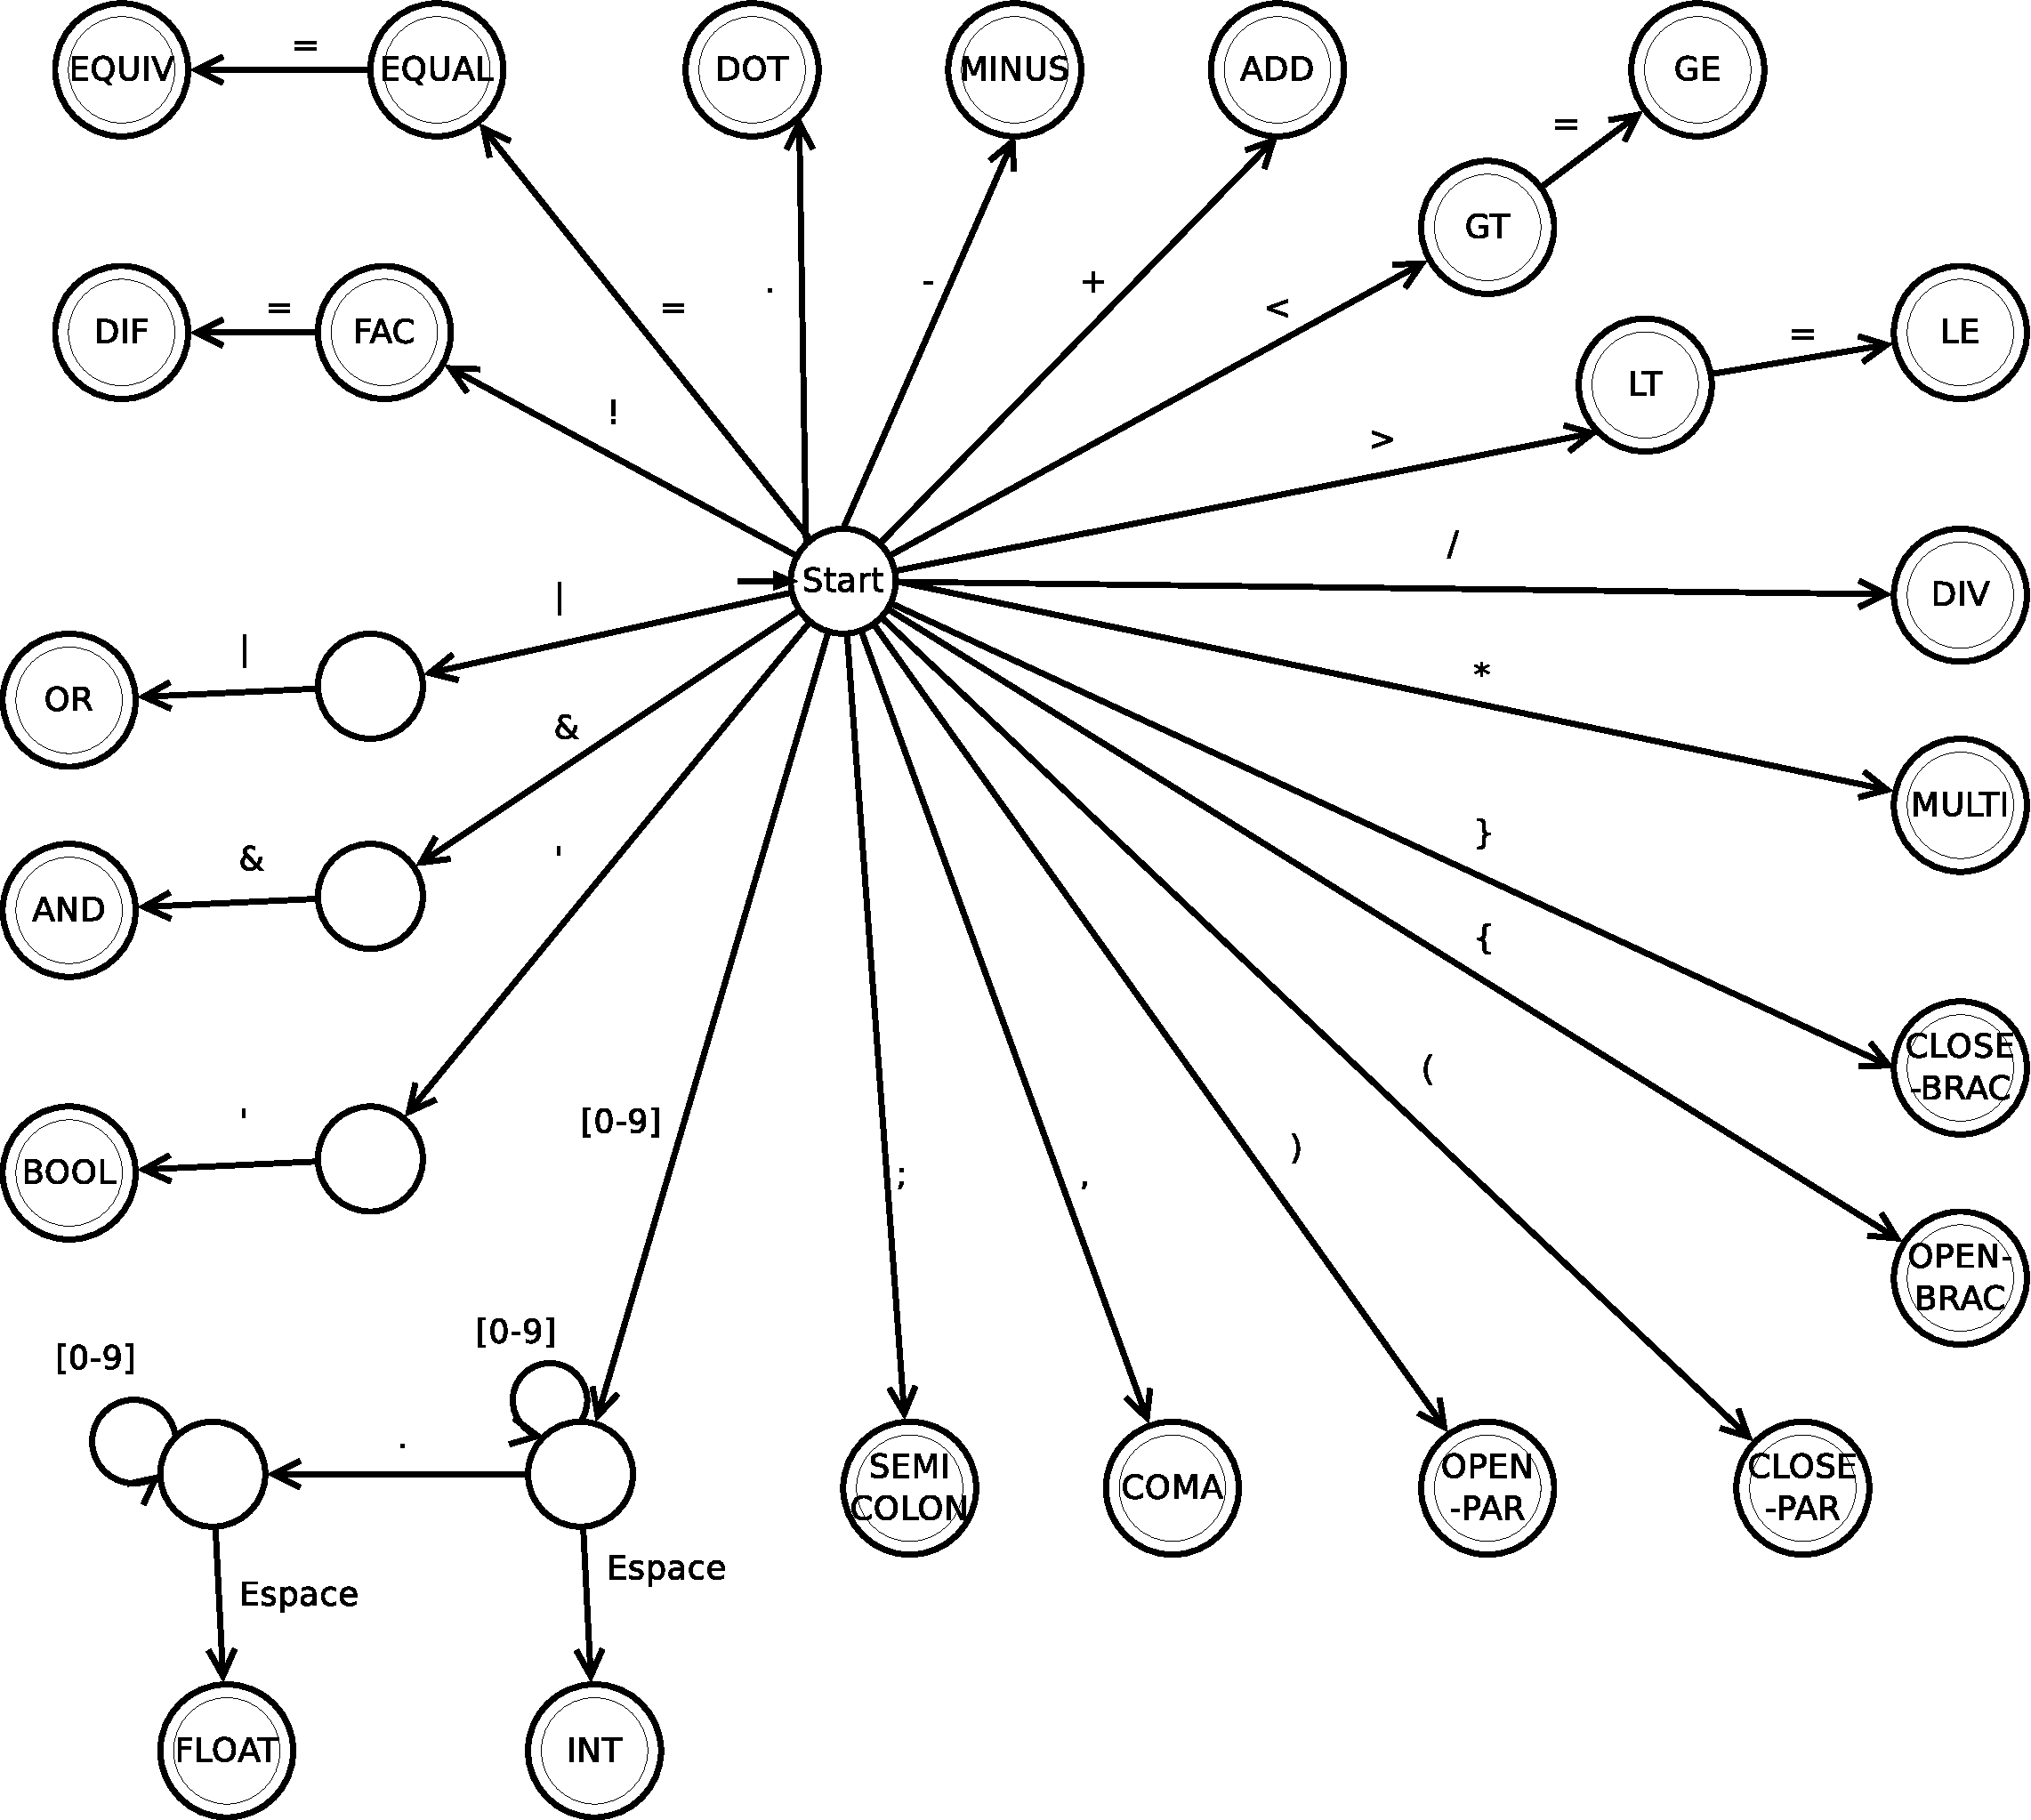
\includegraphics[width=400pt]{automate1.pdf} 
			\caption{automate "non alphabétique"}
			\label{automate1}
	\end{figure}	
  
  
	\begin{figure}[H] \hspace*{-2cm} 
    	\centering
   	  		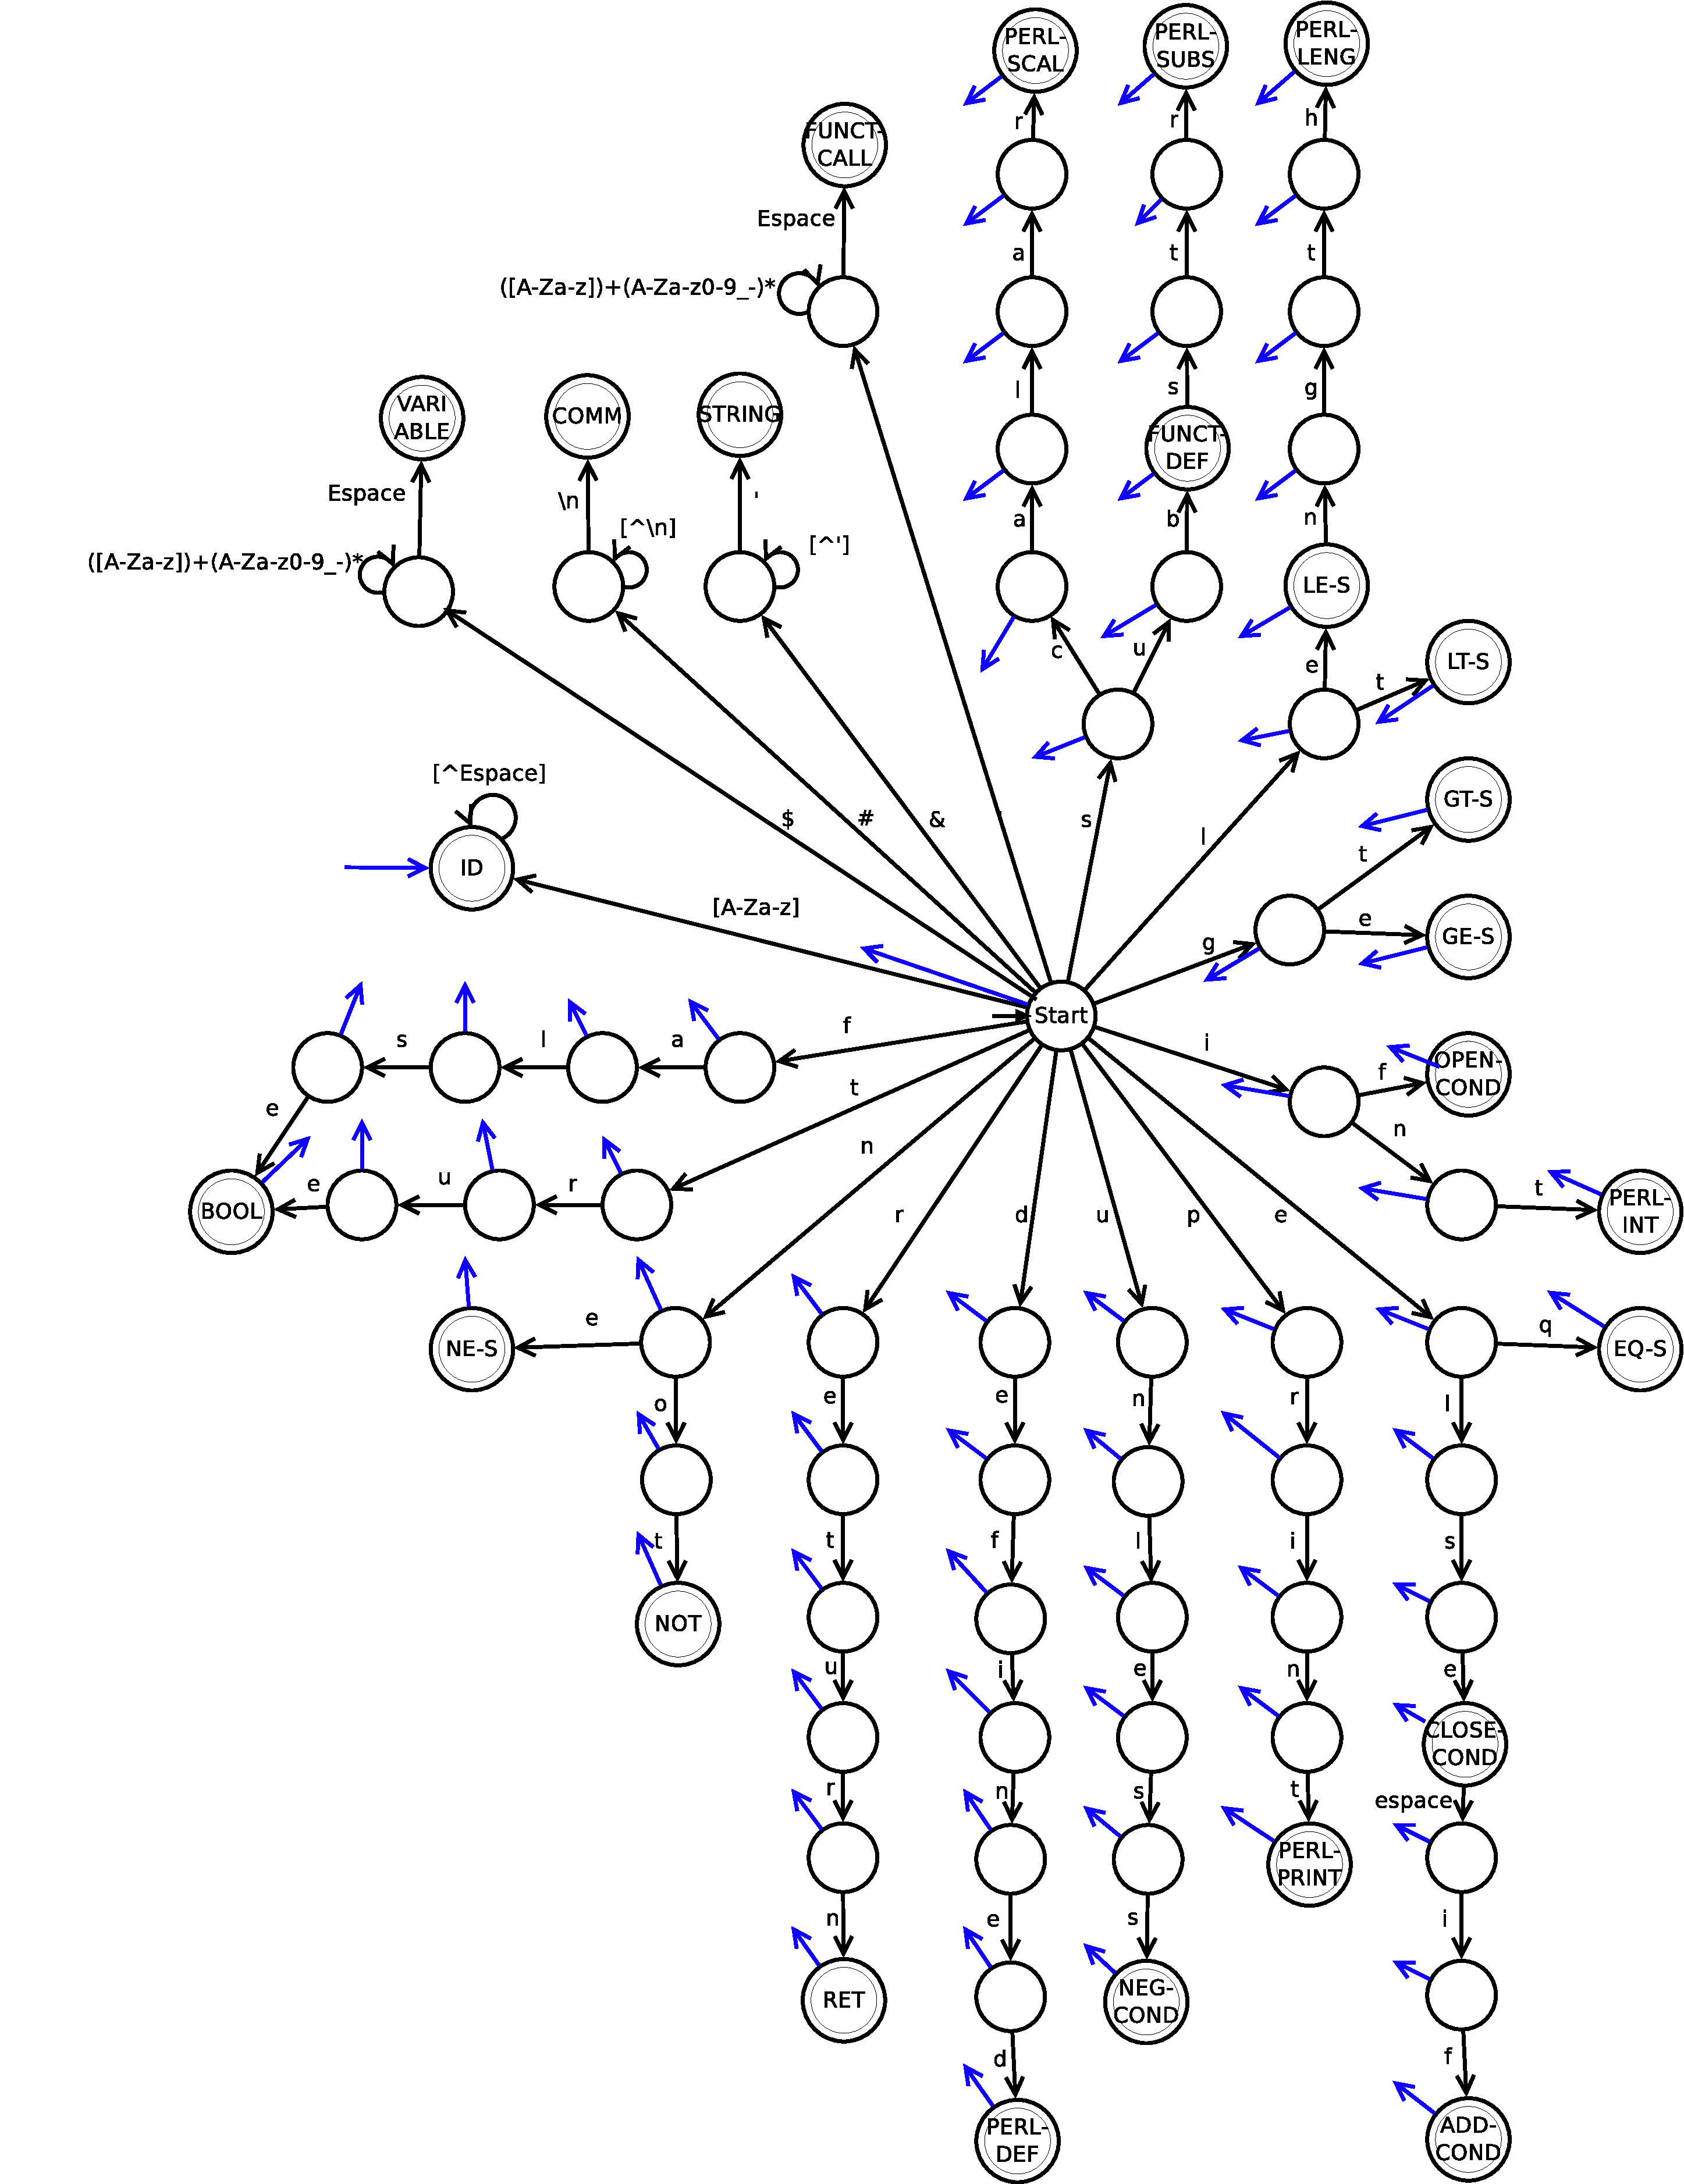
\includegraphics[width=450pt]{automate2.pdf} 
			\caption{automate "alphabétique"}
			\label{automate2}
  	\end{figure}	
	
	\subsubsection{Implémentation}
	Nous définissons une méthode \verb?scans? (de la classe \verb?PerlScanner?) qui reçoit le fichier Perl en paramètre. Celui-ci est alors chargé en mémoire et on appelle la fonction \verb?getNextToken?\\
	Celle-ci reçoit un string en paramètre, puis utilise les regex définies dans les DFA pour reconnaître le premier token du string.\\
	Elle renvoi alors le token (une instance de la classe \verb?Token?) et le string duquel elle a retiré le token.\\
	~\\
	le scanner appelle donc \verb?getNextToken? jusqu'à ce que les strings représentant le document soient vide.\\
	~\\
	Le scanner étant créé en Python, il est très facile de gérer les regex, en utilisant du code comme celui-ci :
\begin{figure}[H]
\fontfamily{pcr}
\begin{lstlisting}
if line[0] == "g":
	if re.match("gt[^a-zA-Z0-9__-]", line):
		line = line[2:]
		return token.token("GT-S", ""), line
	if re.match("ge[^a-zA-Z0-9__-]", line):
		line = line[2:]
		return token.token("GE-S", ""), line
\end{lstlisting}
\fontfamily{}
\caption{Extrait de la méthode getNextToken()}
\label{lst:getNextToken}
\end{figure}

\subsection{Le parser}

Le scanner (l'analyse lexicale) renvoie une liste de lexèmes. Le rôle du parser est alors de vérifier que cette liste respecte la grammaire tout en l'arrangeant en une structure ordonnée (le $parse tree$) basée sur la grammaire. Le parser est du type LL(1), ce qui signifie qu'il part du symbole de départ (ici : \verb?S?) qu'il va transformer itérativement à l'aide de la table d'action et d'un symbole de look-ahead jusqu'à obtenir tous les terminaux de l'input.\\

Notre parser est implémenté en une instance de notre classe \verb?LL1Parser? dont l'attribut \verb?grammar? est une instance de \verb?CFGrammar? représentant la grammaire décrite précédemment. Lors du parsing, il maintient deux structures de données : une liste \verb?output? décrivant les actions effectuées à chaque étape (\verb?M? pour un matching, \verb?Pi? pour l'application de la règle $i$, \verb?A? si l'input est accepté et \verb?E? si l'input est refusé) et un arbre \verb?parseTree? structurant les tokens. Celui-ci est composé de \verb?ParseTreeNode?, contenant une référence vers un token (\verb?value?), une référence vers le noeud père (\verb?father?) et une liste ordonnée de noeuds enfants (\verb?children?). Le parser possède donc également une référence \verb?currentNode? vers le noeud actuel dans le parse tree.\\

Le détail de l'implémentation est donné à l'annexe \ref{anx:parserImpl}. Celle-ci se base sur une fonction récursive qui récupère le noeud actuel dans le parse tree et le premier symbole de l'input restant, puis décide de la règle (ou du matching) à appliquer sur base de la table d'action. Dans le cas où on applique une règle, la fonction s'appelle elle-même pour chaque symbole produit par la règle.\\

Remarque : Notre classe \verb?Parser? fonctionne avec toute grammaire LL(1). D'autres exemples de telles grammaires (inspirées des séances d'exercices) sont données dans le fichier \verb?grammars_examples.py? et des exemples d'utilisations sont donnés dans \verb?parser_test.py?.

\subsection{Transformation en AST}

Étant donné que la grammaire contient de nombreuses règles superflues pour permettre au parser de n'utiliser qu'un seul symbole de look-ahead, le parse tree renvoyé par le parser contient également beaucoup d'informations superflues. Avant de l'utiliser pour générer du code, nous le simplifions donc en un AST (Abstract Syntax Tree) ne contenant que les informations nécessaires à la génération du code.\\

Cette étape, effectuée par notre classe \verb?SyntaxTreeAbstracter? prenant un parse tree en entrée, ressemble fort à une inversion des modifications décrites à la section \ref{sct:gramModif} et consiste majoritairement en de la manipulation des noeuds de l'arbre. Chaque méthode gère un type de noeud particulier et se charge d'appeller la méthode correspondant aux type des fils du noeud donné en paramètre. La figure \ref{lst:ex_STA} montre deux exemples de ces méthodes.

\begin{figure}[H]
\fontfamily{pcr}
\begin{lstlisting}
def abstractFctCall(self, fctCallNode):
	nameNode = fctCallNode.children[0]
	name = nameNode.value.name
	if (name == "FUNCT-NAME"):
		name = nameNode.value.value
	abstractFctCallNode = parseTreeNode(token.token("Fct-Call", value=name))
	# children are the arguments
	for argRoot in fctCallNode.findToken("FUNCT-CALL-ARG", maxDepth=2):
		for firstArgNode in argRoot.findToken("FUNCT-CALL-ARG-BEG"):
			expNode = firstArgNode.children[0]
			abstractFctCallNode.giveNodeChild(self.abstractExp(expNode))
		for nextArgNode in filterargRoot.findToken("FUNCT-CALL-ARG-END"):
			expNode = nextArgNode.children[1]
			abstractFctCallNode.giveNodeChild(self.abstractExp(expNode))
	return abstractFctCallNode

def abstractSimpleExp(self, simpleExpNode):
	simpleExpTypeNode = simpleExpNode.children[0]
	simpleExpType = simpleExpTypeNode.value.name
	if (simpleExpType == "INT" or simpleExpType == "STRING" or simpleExpType == "VARIABLE"):
		return parseTreeNode(token(simpleExpType, value=simpleExpTypeNode.value.value))
	elif (simpleExpType == "FUNCT-CALL"):
		return self.abstractFctCall(simpleExpTypeNode)
	elif (simpleExpType == "OPEN-PAR"):
		return self.abstractExp(simpleExpNode.children[1])
	else:
		raise Exception("Unknown Simple Expression Type : " + str(simpleExpType))
\end{lstlisting}
\fontfamily{}
\caption{Exemples de méthodes du SyntaxTreeAbstracter}
\label{lst:ex_STA}
\end{figure}


\subsection{Génération du code}

	\subsubsection{Implémentation}
	La génération du code consiste à prendre un AST et à le parcourir. En fonction des nœuds rencontrés on écrira alors certaines instructions ASM dans le fichier d'output, en traduisant les instructions représentées dans l'AST en code assembleur correspondant.\\
	~\\
	Le fonctionnement est assez similaire à celui du \verb?SyntaxTreeAbstracter?, on reçoit un AST qu'on parcours récursivement et en fonction du type de nœud rencontré on appellera une fonction le traduisant en code assembleur.\\
	Nous définissons deux strings, \verb?code? et \verb?header? qui contiendront le future code assembleur et seront concaténé à la fin.\\
	Nous mettons dans \verb?header? les données ASM nécessaire au lancement du programme et nous y définissons en global tous les strings rencontrés au cours du parcours de l'AST (la partie \verb?.data? donc).\\
	\verb?code? contiendra donc toutes les instructions assembleurs, d'abord les éventuelles fonctions puis le code du main (la partie \verb?.text?).\\
	~\\
	Le code en lui même est assez simple et suit celui de l'exemple ci-dessous. La vrai difficulté de cette partie était de trouver comment traduire en assembleur les différentes instructions, ce langage étant par nature limité. Nous avons de plus décidé de ne pas importer de fonctions C dans notre code afin de ne pas risquer de problème de librairies manquantes et surtout de conserver uniquement du code assembleur, donc plus optimisé et rapide.\\
	
	\begin{figure}[H]
\fontfamily{pcr}
\begin{lstlisting}
	def instruct_list(self, codeNode):
		for child in codeNode.children:
			if child.value.name =="Cond":
				self.cond(child)
			elif child.value.name =="Assign":
				self.assign(child)
			elif child.value.name =="return":
				self.retur(child)
			elif child.value.name =="Fct-Call":
				self.funct_call(child)
			elif child.value.name !="Instr" and child.value.value !="END":
				raise "instruct-list non valide"
			self.code = self.code +"\n"
				
	def funct_call(self, codeNode):
		if codeNode.value.value == "PERL-PRIN":
			for stringNode in codeNode.children:
				if stringNode.value.name == "STRING":
					self.registerString(stringNode.value.value)
					self.code = self.code + "	/* syscall write	*/ \n"
					self.code = self.code + "	MOV 	R0, #1\n"
					self.code = self.code + "	LDR 	R1, ="+self.listString[stringNode.value.value]+"\n"
					self.code = self.code + "	LDR 	R2, ="+self.listStringLen[stringNode.value.value]+"\n"
					self.code = self.code + "	MOV 	R7, #4\n"
					self.code = self.code + "	SWI 	#0\n"
				else:
					raise "perl-print ne prend que des strings en parametre"
			
		else: # fonctions definies par l utilisateur
\end{lstlisting}
\fontfamily{}
\caption{Extrait de code du générateur de code}
\label{lst:codeGeneration}
\end{figure}


	\subsubsection{Traductions des instructions en code ASM}
		On définit une série de fonctions traduisant une instruction spécifique en code assembleur, souvent ces fonctions s'appellent mutuellement entre elles.\\
		\paragraph{Les expressions}~\\
			Ce sont les opérations de base. On commence par mettre dans deux registres vides les deux paramètres du calcul (ces deux paramètres pouvant nécessiter d'être calculés via un appel de fonction, une autre expression, ... ). Il suffit alors de faire le calcul correspondant à l'expression sur ces deux registres. On renvoi ensuite le (numéro du) registre contenant le résultat. Puis on vide éventuellement les registres si on ne les utilise plus.
				\begin{figure}[H]
\fontfamily{pcr}
\begin{lstlisting}
	MOV 	R0, R5 		
	BL		metA1		
	MOV 	R7, R0		
	MOV 	R8, #3		
	ADD		R9, R7, R8	
\end{lstlisting}
\fontfamily{}
\caption{Exemple d'expression (\$number = \&metA1(\$arg1)+3;) en ASM}
\label{lst:ExExpression}
\end{figure}

		\paragraph{Les assignations}~\\
			On commence par analyser la variable, si elle existe on récupère le registre où elle est stockée (via un dictionnaire ayant en clé le nom de la variable et en valeur son numéro de registre) sinon on lui attribue un nouveau registre libre. Ensuite on calcule la valeur de l'assignation, ce qui peut nécessiter à nouveau d'autres calculs et codes assembleur. L'assignation se résume alors à mettre dans le registre de la variable la valeur du registre contenant le résultat de cette assignation.
				\begin{figure}[H]
\fontfamily{pcr}
\begin{lstlisting}
	SUB		R7, R6, R5
	ADD		R8, R5, R7
	MUL		R7, R4, R8
	MOV 	R4, R7
\end{lstlisting}
\fontfamily{}
\caption{Exemple d'assignation (\$arg1=\$arg1*(\$arg2+(\$arg3-\$arg2));) en ASM}
\label{lst:ExAssignation}
\end{figure}		
		
		\paragraph{Les returns}~\\
			Return fonctionne de la même manière, sauf qu'au lieu de mettre le résultat de l'assignation dans le registre d'une variable, on le met dans le registre 0, conçu pour contenir la valeur de retour des fonctions.
				\begin{figure}[H]
\fontfamily{pcr}
\begin{lstlisting}
	def retur(self, codeNode):
		for child in codeNode.children:
			if child.value.name == "OPERATOR": 
				result = self.expression(child)
				self.code = self.code + "	MOV 	R0, R"+str(result)+"\n"
				if result not in self.listVariable.values():
					self.listRegister[result] = 0					
			elif child.value.name == "STRING": 
				self.registerString(child.value.value)
				self.code = self.code + "	LDR 	R0, ="+self.listString[child.value.value]+"\n"
			elif child.value.name == "INT": 
				self.code = self.code + "	MOV 	R0, #"+child.value.value+"\n"				
			elif child.value.name == "VARIABLE": 
				self.code = self.code + "	MOV 	R0, R"+str(self.getRegisterOfVariable(child.value.value))+"\n"				
			elif child.value.name == "Fct-Call": 
				self.funct_call(child)
				# le resultat est deja ans R0		
			else:
				raise Exception("An error occurs during a return")
\end{lstlisting}
\fontfamily{}
\caption{Fonction calculant les returns}
\label{lst:ExReturn}
\end{figure}
		\paragraph{Les conditions}~\\
			L'AST représente les conditions sous forme d'arbres en ajoutant les else/elsif comme étant un fils du if/elsif précédent. Un élément de la condition contient donc comme fils possibles : 
			\begin{enumerate}
				\item Une expression.\\
					On appelle donc la fonction les analysant.
				\item Une liste d'instruction.\\
					On appelle donc la fonction instruct-list (\ref{instruct-list}).
				\item Un else ou elsif le suivant.\\
					On appelle donc récursivement la fonction gérant les conditions.
			\end{enumerate}
			~\\
			Le principal problème des conditions est qu'elles peuvent être imbriquées. Or en assembleur les conditions sont gérées via des branchements utilisant différents labels. Pour appeler les bons labels on doit donc à chaque fois savoir précisément à quel niveau on se trouve dans l'imbrication des conditions.\\
			On définit deux types de labels :\begin{description}
				\item[else$ab$] : permet de passer au else/elsif suivant (si la condition du if/elsif courant n'est pas remplie)\\
				$a$ est un nombre identifiant dans quel bloc de condition on se trouve.\\
				$b$ est un nombre identifiant à quel niveau on se trouve dans ce bloc.
				\item[end$a$] : permet de quitter les conditions. Si on est rentré dans un des if/elsif, à la fin on saute directement à ce point pour éviter les autres elsif/else défini ensuite.\\
				Il n'y a donc besoin que du nombre identifiant dans quel bloc de condition on se trouve, ce label étant commun à tous le niveau de la condition.
			\end{description}
\begin{figure}[H]
\fontfamily{pcr}
\begin{lstlisting}
	MOV 	R7, #6
	CMP		R4, R7
	BNE else60
	MOV 	R7, #2
	CMP		R5, R7
	BNE else70
	MOV 	R7, #3
	CMP		R6, R7
	BNE else80
	/* syscall write	*/ 

	B end8
else80: 
	MOV 	R7, #3
	CMP		R4, R7
	BNE else81
	/* syscall write	*/ 

	B end8
else81: 
	/* syscall write	*/ 

end8:
	B end7
else70: 
	/* syscall write	*/ 

end7:
	B end6
else60: 
	/* syscall write	*/ 

end6:
\end{lstlisting}
\fontfamily{}
\caption{Exemple de conditions imbriquées en ASM}
\label{lst:ExCond}
\end{figure}

\begin{figure}[H]
\fontfamily{pcr}
\begin{lstlisting}
	if $arg1 == 6 { 
		if $arg2 == 2 {
			if $arg3 == 3 { print ('passage param : ok'); }
			elsif $arg4 == 3 { print ('passage param : erreur'); } 
			else { print ('passage param : erreur'); };
		}
		else { print ('passage param : erreur'); }; }
	else { print ('passage param : erreur'); };
\end{lstlisting}
\fontfamily{}
\caption{Code Perl correspondant au code ASM de la figure \ref{lst:ExCond}}
\label{lst:ExCondSource}
\end{figure}


		\paragraph{les appels de fonctions}~\\
		Ils peuvent être de deux types : \begin{itemize}
			\item Un appel à la fonction perl \verb?print?.\\
				On utilise alors un system call write linux pour gérer cet affichage
\begin{figure}[H]
\fontfamily{pcr}
\begin{lstlisting}
	/* syscall write	*/ 
	MOV 	R0, #1
	LDR 	R1, =str12
	LDR 	R2, =len12
	MOV 	R7, #4
	SWI 	#0
\end{lstlisting}
\fontfamily{}
\caption{Exemple de print en ASM}
\label{lst:ExPrintPerl}
\end{figure}
			
			\item Un appel à une fonction définie dans le code.\\
				Il suffit de mettre dans les registres 0 à 3 les arguments de la fonction. Et d'écrire dans le code assembleur : "BL $<$nom de la fonction$>$".\\
				Le programme ira alors à la première instruction de la fonction. Puis quand celle-ci sera finie, il reviendra automatiquement à l'instruction suivante dans le code appelant.\\
				~\\
				Par manque de temps nous n'avons malheureusement pas eu le temps d'implémenter la gestion de plus de quatre paramètres, cela aurait nécessité d'utiliser le stack, la procédure que nous aurions dû implémenter est décrite à la section \ref{sct:gestionStack}
		\end{itemize}
		
			\paragraph{les listes d'instructions et de fonctions}\label{instruct-list}~\\
				Ces deux parties sont gérées respectivement par \verb?instruct-list? et \verb?funct-list? qui se résument en fait à parcourir ces listes d'instructions ou de fonctions et à appeler les différents méthodes vue ci-dessus.\\
				~\\
				\verb?funct-list? nécessite cependant une instruction supplémentaire à la fin de chaque fonction. Il faut y rajouter "BX	LR" pour quitter la fonction et revenir à l'instruction suivant l'appel de la fonction (cela correspond plus ou moins à "MOV		PC, LR").

	\subsubsection{Variable shadowing}
		Nous profitons également de ce parcours récursif de l'AST pour vérifier que le code ne viole pas certaines règles. En particulier nous vérifions qu'il ne fait pas appel à des variables inaccessibles.\\
		~\\
		Cette vérification se fait en plusieurs étapes. D'abord à chaque création/assignation de variable nous l'ajoutons dans une liste les reprenant toutes, ainsi lors d'un appel nous pouvons aisément vérifier si cette variable a déjà été créée, sinon un message d'erreur apparaîtra.\\
		Ensuite nous sommes particulièrement attentif aux variables utilisées dans les fonctions, afin d'éviter qu'elles n'utilisent des variables du main. Pour cela à chaque appel de fonction, on "push" la liste des variables et on en crée une nouvelle qui ne contient que les variables passées en paramètres.\\
		On peut ainsi vérifier qu'on n'accède qu'aux variables accessibles (c'est-à-dire aux variables stockées dans cette liste). Il suffit de "poper" cette liste à la fin pour retrouver le contexte initiale.\\
		~\\
		Nous utilisons plus ou moins le même principe pour gérer les conditions en créant "plusieurs couches" de stacks (au moyen d'une liste contenant des dictionnaires de variables) : \begin{itemize}
			\item A chaque entrée dans une condition : On crée une couche (donc on ajoute un dictionnaire dans la liste représentant le stack)
			\item A chaque variable créée dans la condition : On l'ajoute à la dernière couche (donc on l'ajoute dans le dernier dictionnaire)
			\item En sortant d'une condition : On supprime le dernière couche (donc on supprime le dernier dictionnaire et les variables qu'il contient)
		\end{itemize}
		Ainsi nous sommes sûr de n'utiliser que des variables vraiment accessibles.\\
		Rem : On utilise des dictionnaires afin de coupler cela avec la position des variables (c'est-à-dire le numéro du registre dans lequel elle se trouve) pour simplifier notre programme. En effet il est très pratique d'utiliser un dictionnaire ayant pour clé la variable et pour valeur son numéro de registre. On peut ainsi vérifier la portée des variables et leur localisation en même temps.\\
		~\\
		Ce système permettrait aussi de gérer les variables globales, qu'on pourrait imaginer être définie dans le code ou avant les listes de fonctions ou instructions. Il suffirait de leur réserver le premier dictionnaire de notre liste de dictionnaire. Ainsi elle seraient accessibles à tout endroit du code, mais vu qu'on parcours la liste par sa fin pour trouver les variables, elles ne seraient trouvées qu'en dernier. En cas de conflit de nom, ce serait donc la variable locale qui serait trouvée en première.\\
		Mais comme les variables globales ne sont pas gérées par notre grammaire, nous ne l'avons pas implémenté.


	\subsubsection{Type checking}
		Sur le même principe, nous vérifions que les fonctions prennent le bon nombre d'argument. Pour cela nous utilisons un dictionnaires contenant comme clé le nom de la fonction et comme valeur son nombre de paramètre. Nous remplissons ce dictionnaire lors de la création des fonctions (dans \verb?funct-list?) puis lors de chaque appel nous vérifions que le nombre de paramètre correspond à celui stocké dans le dictionnaire.

	\subsubsection{Gestion du stack ASM}
		\label{sct:gestionStack}
		Par manque de temps nous n'avons pas eu le temps d'implémenter cette partie, ce qui entraîne certaines limitations : \begin{itemize}
			\item On ne peut utiliser plus de 8 variables en parallèles.
			\item On ne peut passer plus de 4 arguments à une fonction.
		\end{itemize}

		Avec plus de temps, il aurait été possible de gérer cela assez finement. Il aurait suffit de représenter l'état du stack de chaque registre avec une liste (éventuellement toutes regroupées elle-même dans une liste pour plus de facilité.). Lorsqu'on cherche une variable qui ne se trouve pas dans un des registres, on la cherche alors dans les stack de ces différents registres.\\
		On parcours alors les listes jusqu'à trouver cette variables. Une fois trouvée, on "pop" le stack petit à petit, c'est-à-dire qu'on pop la dernière variable du stack, qu'on la déplace dans un registre vide, qu'on pop la variable suivantes, ... jusqu'à ce que la variable qui nous intéresse sorte du stack et se retrouve dans le registre. Permettant ainsi de l'utiliser.\\
		~\\
		Inversement quand on veut un registre vide et qu'ils sont tous occupés, il suffirait de pusher un des registres pour le libérer, la variable "perdue" pouvant être aisément retrouvée par la suite, cela ne prête donc pas à conséquence et permet d'utiliser presque autant de variable que l'on désire (en restant dans les limites matérielles possibles).\\
		~\\
		Encore une fois nous n'avons malheureusement pas eu le temps de finir cette partie.
	
%%%%%%%%%%%%%%%%%%%%%%%%%%%%%%%%%%%%%%%%%%%%%%%%%%%%%%%%%%%%%%%%%%%%%%%%%%%%%%%%%%%%%%%%%%%%%%%%%%%%%%%%%%%%%%%%%%%%%%%%%%%%%%%%%%%%%%%%%%%%%%
%%
%%
%%		Guide d'utilisation
%%
%%
%%
%%%%%%%%%%%%%%%%%%%%%%%%%%%%%%%%%%%%%%%%%%%%%%%%%%%%%%%%%%%%%%%%%%%%%%%%%%%%%%%%%%%%%%%%%%%%%%%%%%%%%%%%%%%%%%%%%%%%%%%%%%%%%%%%%%%%%%%%%%%%%%%%
\section{Guide d'utilisation}

Le programme étant écrit en Python il est aisé de le lancer\footnote{Il nécessite juste d'installer python 2.7}.\\
Une fois dans le dossier, il suffit de lancer la commande :
\begin{center}
	python compilateur.py -v -i  $<$fichier perl$>$
\end{center}
L'option -v est optionnelle, si sélectionnée, le programme affichera dans le terminal le résultat de chaque étape intermédiaire.\\
Le code sera créé dans un fichier de même nom que celui du fichier d'input.\\
~\\
Il est également possible de lancer chaque partie séparément, elle afficheront alors dans le terminal le résultat.
\begin{itemize}
	\item python scanner.py -i $<$fichier perl$>$ 
	\item python parser.py -i $<$fichier perl$>$ 
	\item python syntaxtreeabstracter.py -i $<$fichier perl$>$
	\item python codeGeneration.py -i $<$fichier perl$>$ 
\end{itemize}
~\\
Le code assembleur assembleur ainsi produit a été conçu et tester pour être compiler avec le compilateur \verb?android-ndk-r8d? et tester avec \verb?adb?, via ces commandes (une fois l'émulateur lancé, ou un smartphone android connecté).
\begin{enumerate}
\item	android-ndk-r8d/toolchains/arm-linux-androideabi-4.7/prebuilt/linux-x86/bin/arm-linux-androideabi-as -o program.o program.S
\item	android-ndk-r8d/toolchains/arm-linux-androideabi-4.7/prebuilt/linux-x86/bin/arm-linux-androideabi-ld -s -o exécutable program.o
\item	adb push exécutable /data/local/tmp/
\item	adb shell /data/local/tmp/exécutable
\end{enumerate}
Il suffit de modifier la partie $<$linux-x86$>$ en fonction du système d'exploitation.\\
~\\
Nous avons également inclus un fichier perl contenant des instructions gérées par notre grammaire, ainsi que le fichier assembleur correspondant généré par notre compilateur, dans le dossier \verb?inputTests?

%%%%%%%%%%%%%%%%%%%%%%%%%%%%%%%%%%%%%%%%%%%%%%%%%%%%%%%%%%%%%%%%%%%%%%%%%%%%%%%%%%%%%%%%%%%%%%%%%%%%%%%%%%%%%%%%%%%%%%%%%%%%%%%%%%%%%%%%%%%%%%
%%
%%
%%		ANNEXES
%%
%%
%%
%%%%%%%%%%%%%%%%%%%%%%%%%%%%%%%%%%%%%%%%%%%%%%%%%%%%%%%%%%%%%%%%%%%%%%%%%%%%%%%%%%%%%%%%%%%%%%%%%%%%%%%%%%%%%%%%%%%%%%%%%%%%%%%%%%%%%%%%%%%%%%%%

\pagebreak

\section{Annexes}

\subsection{Méthodes générant les tables First, Follow et la table d'action}

\label{anx:FirstFollowAT}

Comme expliqué précédemment, notre classe \verb?CFGrammar? nous a permis de générer automatiquement les tables $First_1$ et $Follow_1$, ainsi que la table d'action. Voici les méthodes utilisées.

La méthode générant $First_1$ (décrite à la Figure \ref{lst:first_1}) va explorer les applications possibles de règles jusqu'à trouver tous les terminaux obtenables, celle générant $Follow_1$ (Figure \ref{lst:follow_1}) recherche, pour chaque symbole $A$, les éléments de $First_1$ correspondant aux symboles générés après $A$ dans une des règles. Finalement, la dernière méthode (Figure \ref{lst:actionTable}) utilise les deux tables précédentes pour déterminer quelle règle appliquer lorsqu'on doit matcher un symbole à un terminal.

\begin{figure}[H]
\fontfamily{pcr}
\begin{lstlisting}
for A in self.symbols:
	if A in self.terminals:
		first[A] = [A]
stable = False
while not stable:
	stable = True
	for A in self.symbols:
		for rule in (rules beginning with A):
			found_epsilon = True
			current_symbol = 0
			while found_epsilon and current_symbol + 1 < len(rule):
				found_epsilon = False
				current_symbol += 1
				for candidate in first[rule[current_symbol]]:
					if candidate == self.emptySymbol:
						found_epsilon = True
					if candidate not in first[A]:
						stable = False
						first[A].append(candidate)
return first
\end{lstlisting}
\fontfamily{}
\caption{Pseudo-code de la méthode générant la table $First_1$}
\label{lst:first_1}
\end{figure}

\begin{figure}[H]
\fontfamily{pcr}
\begin{lstlisting}
follow = {}
first = self.first_1()
stable = False
while (not stable):
	stable = True
	for rule in self.rules:
		for i, A in enumerate(rule):
			if (i == 0):
				continue
			foundEpsilon = True
			epsilonOffset = 0
			while foundEpsilon:
				foundEpsilon = False
				epsilonOffset += 1
				if i + epsilonOffset >= len(rule):
					candidates = follow[rule[0]]
				else:
					candidates = first[rule[i + epsilonOffset]]
				for candidate in candidates:
					if candidate == self.emptySymbol:
						foundEpsilon = True
					elif candidate not in follow[A]:
						stable = False
						follow[A].append(candidate)
return follow
\end{lstlisting}
\fontfamily{}
\caption{Pseudo-code de la méthode générant la table $Follow_1$}
\label{lst:follow_1}
\end{figure}

\begin{figure}[H]
\fontfamily{pcr}
\begin{lstlisting}
first = self.first_1()
follow = self.follow_1()
M = {}
for i, rule in enumerate(self.rules):
	A = rule[0]
	foundEpsilon = True
	current_symbol = 0
	while foundEpsilon:  # will not loop because follow never contains epsilon
		foundEpsilon = False
		current_symbol += 1
		if current_symbol >= len(rule):
			candidates = follow[A]
		else:
			candidates = first[rule[current_symbol]]
		for candidate in candidates:
			if (candidate == self.emptySymbol):
				foundEpsilon = True
			else:
				M[A][candidate] = i
\end{lstlisting}
\fontfamily{}
\caption{Pseudo-code de la méthode générant la table d'action pour $k = 1$}
\label{lst:actionTable}
\end{figure}

\subsection{Implémentation du parser}

\label{anx:parserImpl}

Notre parser est basé sur l'exemple de parser LL(k) donné dans le syllabus. Notre parser n'utilise pas explicitement de symbole de fin, mais celui-ci est imposé par notre grammaire et ajouté automatiquement par notre scanner. Il est donc traité comme les autres symboles.

\begin{figure}[H]
\fontfamily{pcr}
\begin{lstlisting}
def parse(self, inputText):
	self.input = inputText  # list of symbols
	self.output = []
	self.error = False
	self.success = False

	self.parseTree = parseTreeNode(token(self.grammar.startSymbol))
	self.currentNode = self.parseTree

	self.parse_recursiveCall()
	return self.output

def parse_recursiveCall(self):
	if (self.error or self.accept):
		return
	stack_token = self.currentNode.value
	input_token = self.input[0]  # only one character as we have an LL1-parser
	# notation from the syllabus - pp. 116
	X = stack_token.name
	u = input_token.name

	if (u in self.M[X]):
		self.produce(self.M[X][u])
	elif (X in self.grammar.terminals and X == u):
		self.match()
	else:
		self.trigger_error(X, u)

def trigger_error(self, X, u):
	self.output.append("E")
	if u not in self.grammar.symbols:
		raise ParseError("Unknown symbol", u)
	else:
		raise ParseError("Misplaced symbol", u)

def trigger_accept(self):
	self.output.append("A")
	self.success = True

def produce(self, i):
	self.output.append("P" + str(i))
	saved_current = self.currentNode
	for produced in (symbols produced by rule i):
		if (produced != self.grammar.emptySymbol):
			self.currentNode.giveChild(token(produced))
			self.currentNode = self.currentNode.children[-1]
			self.parse_recursiveCall()
			self.currentNode = saved_current
	self.currentNode = saved_current

def match(self):
	parseTreeToken = self.currentNode.value
	inputToken = self.input.pop(0)
	parseTreeToken.value = inputToken.value
	self.output.append("M")
	if (len(self.input) == 0):
		self.trigger_accept()
\end{lstlisting}
\fontfamily{}
\caption{Pseudo-code du Parser}
\label{lst:parser}
\end{figure}

 
\subsection{Grammaire initiale}\label{gramm-init}

\hspace{-1.0cm}\begin{tabular}{rrl}
1)&$<$PROGRAM$>$		& $\rightarrow$ $<$FUNCT-LIST$>$ $<$INSTRUCT-LIST$>$\\ 
2)&					& $\rightarrow$ $<$FUNCT-LIST$>$\\  
3)&					& $\rightarrow$ $<$INSTRUCT-LIST$>$\\  					
4)&$<$FUNCT-LIST$>$	& $\rightarrow$ $<$FUNCT$>$ \\ 
5)&					& $\rightarrow$ $<$FUNCT-LIST$>$ $<$FUNCT$>$\\ 				
6)&$<$FUNCT$>$			& $\rightarrow$ funct-def id open-par $<$FUNCT-ARG$>$ close-par open-brac \\
&						& $<$INSTRUCT-LIST$>$ close-brac \\  			
7)&$<$FUNCT-ARG$>$		& $\rightarrow$ open-par $<$ARG-LIST$>$ close-par\\  
8)&$<$ARG-LIST$>$		& $\rightarrow$ $<$ARG-LIST$>$ coma variable \\   
9)&					& $\rightarrow$ variable\\   
10)&					& $\rightarrow$ epsilon \\  

11)&$<$INSTRUCT-LIST$>$	& $\rightarrow$ $<$INSTRUCT-LIST$>$ $<$INSTRUCT$>$ semicolon\\ 
12)&					& $\rightarrow$ $<$INSTRUCT$>$ semicolon\\ 
					
13)&$<$FUNCT-CALL$>$	& $\rightarrow$ funct-name $<$FUNCT-CALL-ARG$>$\\ 

14)&$<$FUNCT-CALL-ARG$>$& $\rightarrow$ $<$FUNCT-CALL-ARG$>$ coma $<$EXP$>$\\ 
15)&					& $\rightarrow$ $<$EXP$>$\\ 
16)&					& $\rightarrow$ epsilon\\ 

17)&$<$INSTRUCT$>$		& $\rightarrow$ variable equal $<$EXP$>$\\ 
18)&					& $\rightarrow$ $<$EXP$>$\\
19)&					& $\rightarrow$ ret $<$EXP$>$\\
20)&					& $\rightarrow$ $<$COND$>$\\
					
21)&$<$COND$>$			& $\rightarrow$ open-cond $<$EXP$>$ open-brac $<$INSTRUCT-LIST$>$ close-brac $<$COND-END$>$\\



22)&$<$COND-END$>$		& $\rightarrow$ add-cond $<$EXP$>$ open-brac $<$INSTRUCT-LIST$>$ close-brac $<$COND-END$>$ \\
23)&					& $\rightarrow$ close-cond open-brac $<$INSTRUCT-LIST$>$ close-brac\\
24)&					& $\rightarrow$ epsilon \\
					
25)&$<$SIMPLE-EXP$>$	& $\rightarrow$ int \\
26)&					& $\rightarrow$ $<$FUNCT-CALL$>$ \\
27)&					& $\rightarrow$ variable \\
28)&					& $\rightarrow$ string \\				

29)&$<$EXP$>$			& $\rightarrow$ $<$SIMPLE-EXP$>$   \\
30)&					& $\rightarrow$ open-par $<$EXP$>$ close-par\\ 
31)&					& $\rightarrow$ $<$EXP$>$ add $<$EXP$>$ \\
32)&					& $\rightarrow$ $<$EXP$>$ minus $<$EXP$>$ \\
33)&					& $\rightarrow$ $<$EXP$>$ multi $<$EXP$>$ \\
34)&					& $\rightarrow$ $<$EXP$>$ div $<$EXP$>$ \\
35)&					& $\rightarrow$ $<$EXP$>$ equiv $<$EXP$>$ \\
36)&					& $\rightarrow$ $<$EXP$>$ gt $<$EXP$>$ \\
					
					
\end{tabular}

\subsection{Exemple d'utilisation}
En lançant le code assembleur obtenu à partir du code perl contenu dans le dossier \verb?inputTests?, nous obtenons : 
 \begin{figure}[H] \hspace*{-2cm} 
   \centering
   	  %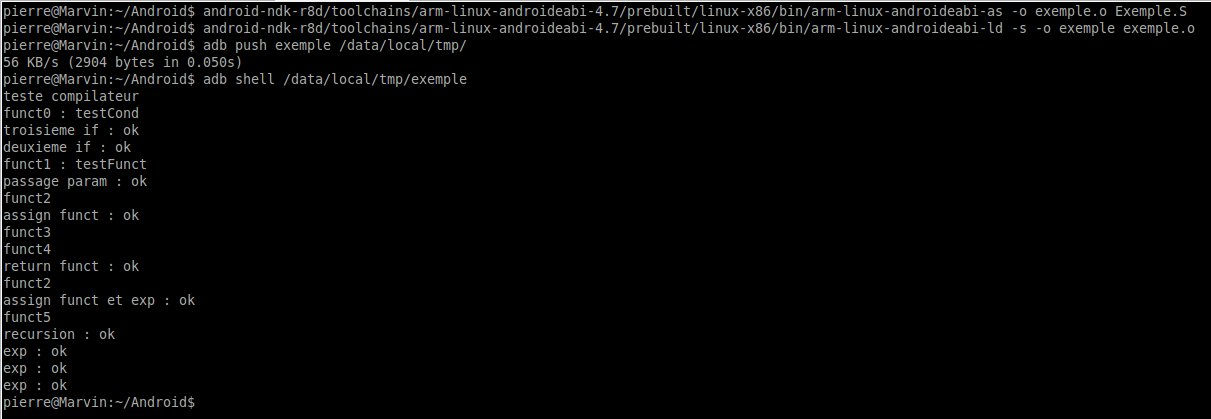
\includegraphics[width=375pt]{exemple.jpg} 
   	  exemple.jpg
			\caption{Exemple d'utilisation}
			\label{ExempleUtilisation}
 \end{figure}	

\end{document}